% Overleaf compiler: XeLaTeX. The report is maintained directly in this file.
\documentclass[a4paper,12pt]{article}
\usepackage{fontspec}
\usepackage{polyglossia}
\setmainlanguage{russian}
\setotherlanguage{english}
\IfFontExistsTF{DejaVu Serif}{\setmainfont{DejaVu Serif}}{\setmainfont{Times New Roman}}
\IfFontExistsTF{DejaVu Sans}{\setsansfont{DejaVu Sans}}{\setsansfont{Arial}}
\IfFontExistsTF{DejaVu Sans Mono}{\setmonofont{DejaVu Sans Mono}}{\setmonofont{Consolas}}
\usepackage{amsmath,amssymb}
\usepackage[left=25mm,right=20mm,top=20mm,bottom=22mm]{geometry}
\usepackage{graphicx,float,booktabs,tabularx,array}
\usepackage{caption,subcaption}
\usepackage{enumitem}
\usepackage{fancyhdr}
\usepackage[hidelinks]{hyperref}
\usepackage{xurl}
\hypersetup{hypertexnames=false}
\usepackage{microtype}
\setlength{\parindent}{1.25cm}
\setlength{\parskip}{0.2em}
\setlength{\headheight}{15pt}
\emergencystretch=3em
\renewcommand{\arraystretch}{1.18}
\captionsetup{font=small,labelfont=bf}
\setlist{leftmargin=1.2cm,itemsep=0.15em,topsep=0.3em}
\pagestyle{fancy}
\fancyhf{}
\fancyhead[L]{\small Алгоритмы компьютерной графики}
\fancyhead[R]{\small Лабораторная работа № 3}
\fancyfoot[C]{\thepage}
\renewcommand{\headrulewidth}{0pt}
\newcommand{\code}[1]{\nolinkurl{#1}}
\newcommand{\Le}{L_{\mathrm e}}
\newcommand{\Lv}{L_{\mathrm v}}
\newcommand{\TestsCount}{24}
\newcommand{\resultgrid}[1]{%
  \begin{figure}[H]\centering
  \begin{subfigure}{0.44\textwidth}\centering
    \includegraphics[width=\linewidth]{results/#1/image_1.png}
    \caption{Спектральный расчёт}
  \end{subfigure}\hfill
  \begin{subfigure}{0.44\textwidth}\centering
    \includegraphics[width=\linewidth]{results/#1/image_2.png}
    \caption{Расчёт RGB сцены}
  \end{subfigure}
  \par\medskip
  \begin{subfigure}{0.44\textwidth}\centering
    \includegraphics[width=\linewidth]{results/#1/image_1_gray.png}
    \caption{Серый из image\_1}
  \end{subfigure}\hfill
  \begin{subfigure}{0.44\textwidth}\centering
    \includegraphics[width=\linewidth]{results/#1/image_2_gray.png}
    \caption{Серый из image\_2}
  \end{subfigure}
  \caption{Два метода и серые версии при разрешении $600\times600$}
  \end{figure}}

\begin{document}
\begin{titlepage}
  \thispagestyle{empty}
  \begin{center}
    \textbf{МИНИСТЕРСТВО НАУКИ И ВЫСШЕГО ОБРАЗОВАНИЯ РФ}\\[0.6em]
    \textbf{УНИВЕРСИТЕТ ИТМО}\\[0.6em]
    Факультет программной инженерии и компьютерной техники
    \vfill
    {\Large\bfseries ОТЧЁТ ПО ЛАБОРАТОРНОЙ РАБОТЕ № 3}\\[1.2em]
    {\large по дисциплине «Алгоритмы компьютерной графики»}\\[2em]
    {\Large\bfseries Моделирование цветных изображений\\[0.35em]
    Спектральный и RGB расчёт сферы}
    \vfill
    Выполнили: Чжун Ц. Чэнь Х.\\
    Группы: P3310, P3316\\
    Преподаватель: Потемин Игорь Станиславович
    \vfill
    Санкт-Петербург\\2026
  \end{center}
\end{titlepage}

\tableofcontents
\clearpage
\section{Цель и постановка задачи}

Цель работы заключается в расчёте и визуализации распределения яркости цветной диффузной сферы, освещённой точечными источниками с ламбертовской диаграммой и заданными спектрами. Для одной геометрии сравниваются спектральный расчёт и расчёт сцены, заранее преобразованной в CIE RGB.

Приложение реализует обе требуемые последовательности. Первая сохраняет в памяти абсолютное спектральное изображение, затем абсолютные XYZ и RGB, после чего записывает \code{image_1.png}. Вторая использует RGB источников и RGB коэффициент материала и записывает \code{image_2.png}. Выполняются опыты с белыми и цветными источниками. Для каждой пары сохраняются серые версии, показатели различия изображений, три контрольные точки и экстремумы.

\begin{table}[H]\centering\small
\caption{Диапазоны входных данных}
\begin{tabularx}{\textwidth}{@{}lX@{}}\toprule
Параметр & Допустимые значения\\\midrule
Размеры экрана $W,H$ & $100$--$10000$ мм\\
$W_{res},H_{res}$ & $200$--$800$ пикселей, квадратный пиксель\\
$x_L,y_L,x_C,y_C$ & От $-10000$ до $10000$ мм\\
$z_L$ & От $-10000$ до $10000$ мм\\
$z_C$ & От $0$ до $10000$ мм\\
$I_0$ & $0{,}01$--$10000$ Вт/ср\\
Спектральная сетка & $380,390,\ldots,780$ нм, 41 отсчёт\\
$k_d(\lambda)$ & От $0$ до $1$ для каждого отсчёта\\\bottomrule
\end{tabularx}
\end{table}

Наблюдатель $O=(0,0,z_O)$ и источники должны находиться вне сферы. Вся сфера должна помещаться в поле зрения. Входные спектры задаются таблицами, число источников задаётся длиной списка и не ограничено двумя.

Геометрия вводится в миллиметрах. В законе обратных квадратов используется расстояние в метрах. Спектральная яркость $L_\lambda$ измеряется в Вт/(м$^2\cdot$ср$\cdot$нм), интегральная энергетическая яркость $\Le$ --- в Вт/(м$^2\cdot$ср). Фотометрическая яркость вычисляется отдельно как $\Lv=683Y$, кд/м$^2$. Экранные числа $0$--$255$ не являются этими физическими величинами.

\clearpage
\section{Схемы исходного задания}

\begin{figure}[H]\centering
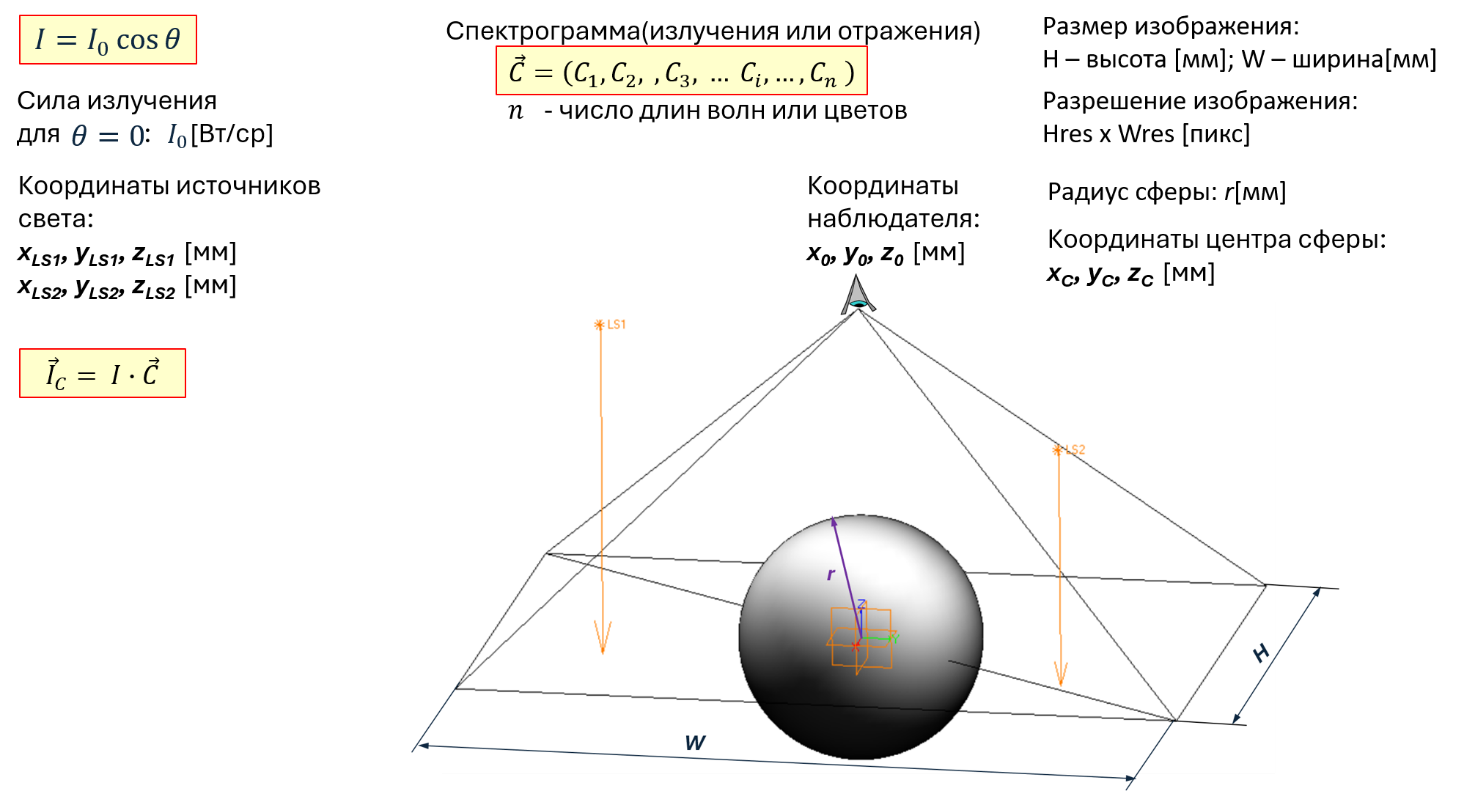
\includegraphics[width=0.96\textwidth]{figures/reference_scene.png}
\caption{Исходная геометрия, спектрограммы и диаграмма источника}
\label{fig:scene}
\end{figure}
\begin{figure}[H]\centering
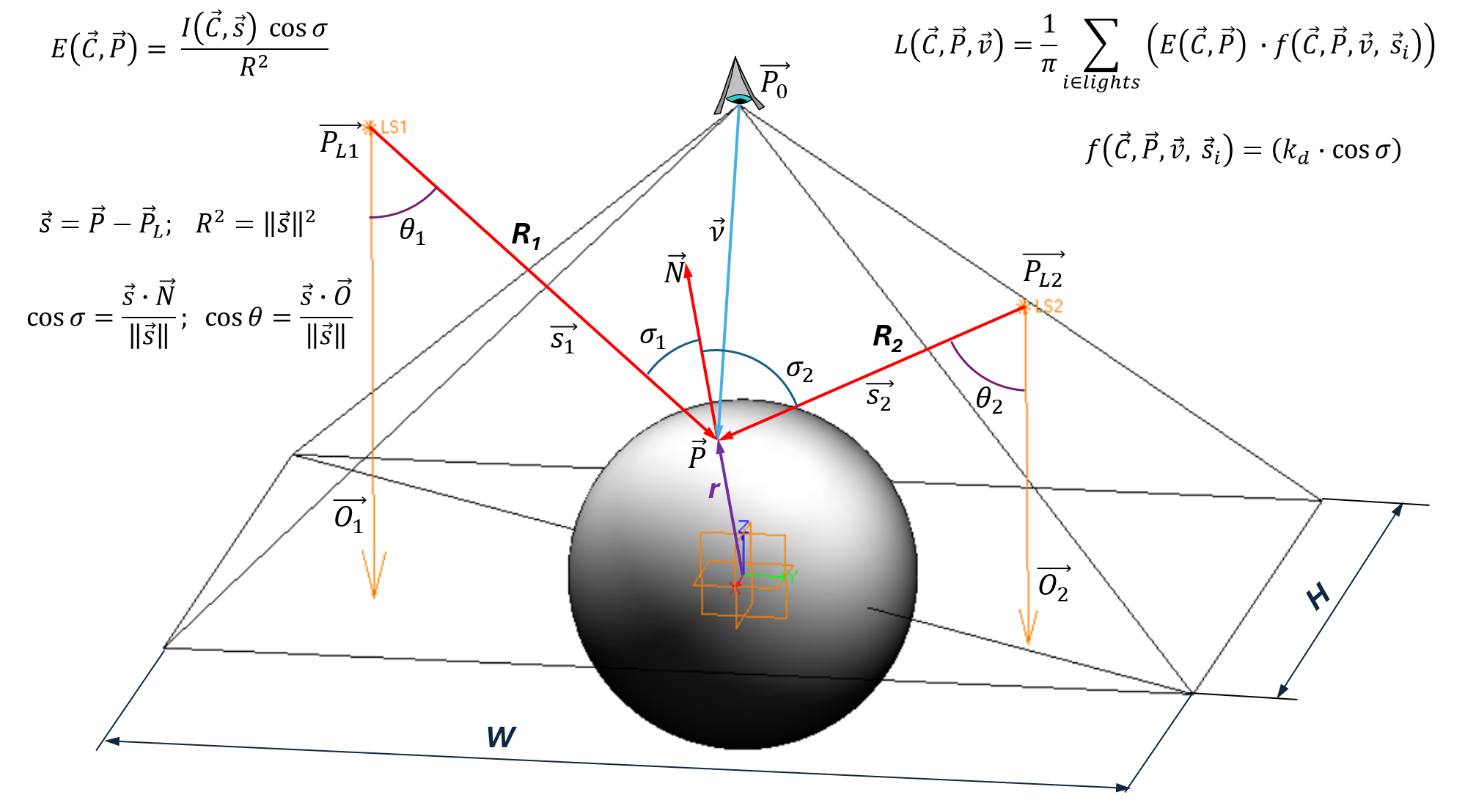
\includegraphics[width=0.96\textwidth]{figures/reference_formula.png}
\caption{Расчёт освещения и отражения в обозначениях задания}
\label{fig:formula}
\end{figure}

На рисунке~\ref{fig:formula} множитель $\cos\sigma$ присутствует и в $E$, и в $f$. Основной режим сохраняет это двойное вхождение и внешний множитель $1/\pi$. Направление приёма задаётся от поверхности к источнику, а нормаль направлена наружу. Это устраняет противоречие знака в исходной подписи вектора $\vec s$.

\clearpage
\section{Геометрия камеры и формула освещения}
\subsection{Перспективная камера и пересечение}

Из единичного направления наблюдения $\vec d$ строится ортонормированный базис $\vec e_r,\vec e_u,\vec d$. Центр экрана лежит на оптической оси на расстоянии $f>0$. По умолчанию $f=(z_{screen}-z_O)/d_z$. Параметр \code{screen_distance_mm} непосредственно задаёт расстояние вдоль оси и позволяет использовать также горизонтальное направление.
\[
 x_j=-\frac{W}{2}+\frac{(j+1/2)W}{W_{res}},\qquad
 y_i=\frac{H}{2}-\frac{(i+1/2)H}{H_{res}}.
\]
\[
 \vec q_{ij}=\frac{f\vec d+x_j\vec e_r+y_i\vec e_u}
 {\|f\vec d+x_j\vec e_r+y_i\vec e_u\|}.
\]
Для луча $P=O+t\vec q$ используются
\[
 b=\vec q\cdot(O-C),\quad c=\|O-C\|^2-R^2,\quad D=b^2-c,
 \qquad t=-b-\sqrt D.
\]
При $D<0$ или $t\leq0$ пиксель относится к фону. Иначе выбирается ближайшее положительное пересечение и $\vec n=(P-C)/R$. Независимая маска отличает фон от неосвещённой поверхности. Полный силуэт проверяется расстояниями от центра до четырёх боковых плоскостей поля зрения.

\subsection{Соответствие формуле рисунка}
Для источника $i$ определены
\[
 r_i=\|P_{L_i}-P\|,\quad \vec l_i=\frac{P_{L_i}-P}{r_i},\quad
 c_{\theta i}=\max(\vec a_i\cdot(-\vec l_i),0),\quad
 c_{\sigma i}=\max(\vec n\cdot\vec l_i,0).
\]
Нормированная ось излучения $\vec a_i$ задаёт диаграмму $I=I_0\cos\theta$. По формулам задания
\[
 E_{i,\lambda}=\frac{I_{0i}S_i(\lambda)c_{\theta i}c_{\sigma i}}{r_i^2},
 \qquad f_{i,\lambda}=k_d(\lambda)c_{\sigma i},
\]
поэтому основной режим \code{reference_diagram} вычисляет
\begin{equation}
 L_\lambda(P)=\sum_i
 \frac{I_{0i}S_i(\lambda)k_d(\lambda)c_{\theta i}c_{\sigma i}^{\,2}}
 {\pi r_i^2}.
 \label{eq:radiance}
\end{equation}
В исходной схеме $\vec s=P-P_L$, но внешняя нормаль нарисована наружу. Использование $\vec l=-\vec s/\|\vec s\|$ согласует приёмный косинус с освещённой стороной. На задней стороне вклад равен нулю.

Дополнительный режим \code{lambert} использует стандартный диффузный закон с одной степенью $c_\sigma$. Основные результаты получены по формуле~\eqref{eq:radiance}, зеркальная составляющая из лабораторной работы 2 исключена.

\clearpage
\section{Спектральные данные и цветовые координаты}
\subsection{Таблицы и абсолютная нормировка}

Таблица преподавателя \code{CIE_XYZ_1931_10nm.xls} содержит функции $\bar x,\bar y,\bar z$ в столбцах D:G листа XYZ. Фактический шаг исходных строк составляет 5 нм. Для программы выбраны существующие строки с шагом 10 нм без интерполяции. Округления и нули преподавательской таблицы сохранены.

В \code{cie_xyz_1931.csv} записаны 41 строка цветовых функций. Файл \code{light_spectra.csv} содержит относительные спектры D65, красного и синего источников, а также исходный спектр чёрного тела 6500 К. Файл \code{reflectance.csv} содержит $k_d(\lambda)$. Значения D65 получены из официальной таблицы CIE с исходным шагом 1 нм. Чёрное тело 6500 К не переименовывается в D65, поскольку одинаковая близкая цветовая температура не означает одинаковый спектр.

Для составной формулы трапеций
\[
 w_0=w_{40}=5\text{ нм},\quad w_1=\cdots=w_{39}=10\text{ нм},
 \qquad S_i(\lambda_j)=\frac{s_i(\lambda_j)}{\sum_k w_ks_i(\lambda_k)}.
\]
Таким образом, $\sum_jw_jS_i(\lambda_j)=1$, и $I_0$ означает интегральную осевую силу излучения во всём принятом диапазоне. Масштаб исходного спектра не меняет результат. Отрицательные, нечисловые и полностью нулевые спектры источника отклоняются.

\subsection{XYZ и CIE RGB 1931}
Переход от абсолютного спектра выполняется по формулам
\[
 X=\sum_jw_jL_{\lambda_j}\bar x_j,\quad
 Y=\sum_jw_jL_{\lambda_j}\bar y_j,\quad
 Z=\sum_jw_jL_{\lambda_j}\bar z_j.
\]
Введём $T(S)=N\,XYZ(S)$, где заданная в работе матрица равна
\[
 N=\begin{bmatrix}
 2.36461&-0.89654&-0.46807\\
 -0.51517&1.42641&0.08876\\
 0.00520&-0.01441&1.00920
 \end{bmatrix}.
\]
Это CIE RGB 1931, а не мониторный sRGB. Знаковые значения RGB сохраняются без обрезания.

Прямая матрица в задании содержит внешний коэффициент $1/0{,}17697$ и не является обратной к приведённой $N$: произведение близко к $5{,}6507I$. Программа сохраняет явно заданный переход XYZ в RGB и использует $N^{-1}$ для обратного направления. Смешивание несовместимых масштабов исключено.

\clearpage
\section{Две последовательности расчёта цвета}
\subsection{Спектральная сцена и image\_1}

Для каждой видимой точки вычисляется весь вектор $L_\lambda$ из 41 значения. Он остаётся в памяти в массиве \code{float64} размером $H_{res}\times W_{res}\times41$. Затем вычисляются XYZ и CIE RGB.
\[
 \text{Спектральная сцена}\longrightarrow L_\lambda(P)
 \longrightarrow XYZ_1(P)\longrightarrow RGB_1(P)
 \longrightarrow \text{image\_1}.
\]
Спектральный куб, XYZ и знаковый RGB не зависят от экспозиции. Они сохраняются вместе с маской и координатами поверхности в \code{radiance_data.npz}. Для проверки абсолютных величин используются
\[
 \Le(P)=\sum_jw_jL_{\lambda_j}(P),\qquad
 \Lv(P)=683Y(P).
\]

\subsection{RGB сцена и image\_2}

Спектры источников переводятся в CIE RGB до обхода пикселей. Материал преобразуется по D65 именно способом, указанным в задании:
\[
 C_i=T(S_i),\qquad
 K_{RGB}=\frac{T(D65\,k_d)}{T(D65)}.
\]
Деление и умножение здесь поканальные. При
\[
 g_i(P)=\frac{I_{0i}c_{\theta i}c_{\sigma i}^{\,2}}{\pi r_i^2}
\]
второе изображение вычисляется независимо от спектральной свёртки пикселя:
\[
 RGB_2(P)=K_{RGB}\odot\sum_i g_i(P)C_i.
\]
Полученный $K_{RGB}$ не ограничивается дополнительно диапазоном $[0,1]$. Он является отношением координат цвета. Физическое ограничение $[0,1]$ применяется к исходному спектральному $k_d$.

\subsection{Условие совпадения}

Если все источники имеют форму D65, то
\[
 T(S_{D65})\odot\frac{T(D65\,k_d)}{T(D65)}
 =T(S_{D65}\,k_d).
\]
Два расчёта поэтому совпадают с точностью арифметики. При других спектрах равенство обычно нарушается: линейное преобразование $T$ сохраняет суммы, но не произвольные поканальные произведения спектров. Различие при цветных источниках является результатом сравнения моделей.

\clearpage
\section{Экранное изображение и серые версии}
\subsection{Одна экспозиция для пары изображений}

Каждое абсолютное CIE RGB изображение сначала преобразуется обратно в XYZ, затем в линейный sRGB:
\[
 c_k=A N^{-1}RGB_k,\qquad
 A=\begin{bmatrix}
 3.2406&-1.5372&-0.4986\\
 -0.9689&1.8758&0.0415\\
 0.0557&-0.2040&1.0570
 \end{bmatrix}.
\]
Для одной пары используется общий максимум по всем видимым пикселям и всем каналам:
\[
 M=\max(0,\max c_1,\max c_2),\qquad
 a=\begin{cases}1/M,&M>0,\\0,&M=0.\end{cases}
\]
Обе карты используют один и тот же $a$. Отдельная нормировка каждого изображения или каждого канала могла бы скрыть различие амплитуд. Белый и цветной варианты имеют собственные пары экспозиций, а их физические величины сравниваются до нормировки.

Перед записью применяется ограничение охвата $u=\operatorname{clip}(ac,0,1)$ и стандартная передаточная функция
\[
 F(u)=\begin{cases}
 12.92u,&u\leq0.0031308,\\
 1.055u^{1/2.4}-0.055,&u>0.0031308,
 \end{cases}
 \qquad G=\operatorname{round}(255F(u)).
\]
Пик общего максимального положительного канала достигает 255. Отрицательные и выходящие за охват координаты обрезаются только для отображения. Их исходные значения остаются в абсолютных массивах, число затронутых пикселей записывается в JSON.

\subsection{Перевод полученного изображения в серый}

Серые изображения вычисляются из фактически записываемых восьмибитных RGB чисел. Сначала применяется $F^{-1}$, затем линейная яркостная строка матрицы $A^{-1}$, после чего снова $F$ и округление до одного канала $0$--$255$.
\[
 Y_{display}=(A^{-1})_{2,:}\,F^{-1}(G/255),\qquad
 G_{gray}=\operatorname{round}(255F(Y_{display})).
\]
Такая серая карта служит для просмотра. Абсолютная $\Lv=683Y$ рассчитывается до экспозиции, ограничения охвата и восьмибитного округления.

\clearpage
\section{Исходные данные демонстрационных вариантов}

\begin{table}[H]\centering\small
\caption{Общие параметры двух опытов}
\begin{tabularx}{\textwidth}{@{}lX@{}}\toprule
Величина & Значение\\\midrule
Экран $W\times H$ & $1200\times1200$ мм\\
Разрешение & $600\times600$ пикселей\\
Наблюдатель $O$ & $(0,0,2500)$ мм\\
Направление и экран & $\vec d=(0,0,-1)$, $z_{screen}=0$ мм\\
Центр и радиус & $C=(0,0,600)$ мм, $R=350$ мм\\
Модель & \code{reference_diagram}, $\cos^2\sigma/\pi$\\
Материал & $k_d=0.08+0.8\exp[-(\lambda-540)^2/(2\cdot45^2)]$\\\bottomrule
\end{tabularx}
\end{table}
\begin{table}[H]\centering\small
\caption{Ламбертовские точечные источники}
\begin{tabular}{@{}clrl@{}}\toprule
Источник & Координаты, мм & $I_0$, Вт/ср & Ось $\vec a$\\\midrule
$L_1$ & $(-650,450,1700)$ & 100 & $(0,0,-1)$\\
$L_2$ & $(550,-250,1600)$ & 70 & $(0,0,-1)$\\\bottomrule
\end{tabular}
\end{table}

Физический размер пикселя равен 2 мм по обеим осям. Перспективный радиус силуэта равен
\[
 \frac{2500\cdot350}{\sqrt{1900^2-350^2}}
 =468.544609\text{ мм}<600\text{ мм}.
\]
Полная сфера помещается в экран. В белом опыте обе таблицы источников равны D65. В цветном опыте используются относительные формы
\[
 s_1(\lambda)=\exp\!\left[-\frac{(\lambda-620)^2}{2\cdot35^2}\right],\qquad
 s_2(\lambda)=\exp\!\left[-\frac{(\lambda-470)^2}{2\cdot25^2}\right].
\]
Геометрия и материал одинаковы, после чтения каждая форма интегрально нормируется.

\begin{table}[H]\centering\small
\caption{Выбранные строки входных спектров}
\begin{tabular}{@{}rrrrr@{}}\toprule
$\lambda$, нм & $k_d$ & D65 & $s_1$ & $s_2$\\\midrule
380 & 0.0814 & 49.9755 & 0.0000 & 0.0015\\
480 & 0.4089 & 115.9230 & 0.0003 & 0.9231\\
530 & 0.8605 & 107.6890 & 0.0367 & 0.0561\\
580 & 0.6189 & 95.7880 & 0.5205 & 0.0001\\
630 & 0.1883 & 83.2886 & 0.9600 & 0.0000\\
780 & 0.0800 & 63.3828 & 0.0000 & 0.0000\\\bottomrule
\end{tabular}
\end{table}
Полные 41-строчные таблицы хранятся в трёх CSV пакета. Фактические спектры каждого опыта вместе со всеми параметрами сцены записываются в \code{results.json}.

\clearpage
\section{Структура приложения и алгоритм}

Программа разделена на небольшой пакет \code{lab3_color_sphere}. Геометрическая основа лабораторной работы 2 сохранена, физические и цветовые операции отделены от интерфейса.
\begin{table}[H]\centering\small
\caption{Назначение модулей}
\begin{tabularx}{\textwidth}{@{}lX@{}}\toprule
Модуль & Ответственность\\\midrule
\code{main.py} & Запуск GUI или пакетного расчёта, аргументы командной строки\\
\code{geometry.py} & Параметры, базис камеры, луч и сфера, видимость и геометрические множители\\
\code{spectral.py} & Три CSV, сетка 41 отсчёта, нормировка спектров, пресеты и ввод сцены\\
\code{color_conversion.py} & Спектр в XYZ и CIE RGB, D65 коэффициент, sRGB и серая версия\\
\code{rendering.py} & Два способа расчёта, контрольные точки, статистика и экспорт\\
\code{gui.py} & Параметры сцены, таблица спектров, расчёт, четыре изображения и сохранение\\\bottomrule
\end{tabularx}
\end{table}

\begin{enumerate}
\item Прочитать входные параметры и спектральные таблицы. Проверить диапазоны, конечность значений и квадратность пикселей.
\item Построить лучи через центры пикселей и найти ближайшую поверхность. Создать отдельную геометрическую маску.
\item Нормировать спектры, заранее вычислить цвета источников и материал $K_{RGB}$ по D65.
\item Для блоков видимых точек рассчитать геометрические множители, полный спектр, XYZ, $RGB_1$ и независимо $RGB_2$.
\item Рассчитать физические яркости, общую экспозицию пары, два RGB изображения, серые версии и разность.
\item Непосредственно по формулам получить три контрольные точки, пиксельные экстремумы и отдельную угловую выборку всей сферы.
\item Записать изображения PNG, таблицы CSV, параметры и статистику JSON, абсолютные массивы NPZ.
\end{enumerate}

Из каталога проекта интерфейс запускается командой
\begin{quote}\small\ttfamily python -m lab3\_color\_sphere.main\end{quote}
Поддерживается также прямой запуск \texttt{python lab3\_color\_sphere/main.py}. Для двух стандартных опытов используется
\begin{quote}\small\ttfamily python -m lab3\_color\_sphere.main --no-gui --case both\end{quote}
Собственные параметры и спектры задаются через \code{--config} и \code{--spectra}. Режим \texttt{--model lambert} выбирает один приёмный косинус. Нужны только NumPy, Pillow и стандартный Tkinter для GUI. Полный спектральный куб \code{float64} при $600^2$ занимает 118080000 байт, при $800^2$ --- 209920000 байт. Блочная обработка ограничивает только промежуточную память.

\clearpage
\section{Результаты при белых источниках}
\resultgrid{white}

В опыте D65 абсолютная разность CIE RGB не превышает $1.4211\cdot10^{-14}$. Два PNG совпадают во всех пикселях, средняя абсолютная разность каналов MAE равна нулю. Это соответствует аналитическому условию совпадения при спектре калибровки материала.

Общий максимум линейного sRGB равен $7.21767609$, экспозиция $a=0.13854875$. Ограничение охвата не затрагивает пиксели обеих карт. Различия между абсолютным спектральным образом и мониторными значениями сохранены в отдельных массивах.

\clearpage
\section{Результаты при цветных источниках}
\resultgrid{colored}

При цветных источниках различаются 171781 видимый пиксель. MAE составляет $8.517839$, RMSE --- $10.884252$, максимальная поканальная разность равна 49 из 255. Оба изображения имеют одну экспозицию, поэтому различие не вызвано отдельным растяжением диапазона.

Общий максимум линейного sRGB равен $12.42716049$, экспозиция $a=0.08046891$. Ограничение охвата затрагивает 115290 пикселей первого и 114798 пикселей второго изображения. Для численного сравнения доступны исходные знаковые CIE RGB и XYZ до ограничения.

\clearpage
\section{Контрольные точки и экстремумы}

Три точки задаются через нормали $\vec n_1=(0,0,1)$, $\vec n_2=(-0.6,0,0.8)$, $\vec n_3=(0.6,0,0.8)$. Их координаты равны $(0,0,950)$, $(-210,0,880)$ и $(210,0,880)$ мм. Точки принадлежат сфере и видимы. Значения рассчитаны непосредственно по формулам, без чтения ближайшего пикселя. Для другой камеры нормали строятся относительно наблюдателя, при необходимости угол уменьшается для сохранения видимости.

\begin{table}[H]\centering\small
\caption{Белые источники D65}
\begin{tabular}{@{}lrrr@{}}\toprule
Точка & $\Le$, Вт/(м$^2\cdot$ср) & $\Lv{}_1$, кд/м$^2$ & $\Lv{}_2$, кд/м$^2$\\\midrule
$P_1$ & 6.798669 & 2652.985 & 2652.985\\
$P_2$ & 6.463882 & 2522.344 & 2522.344\\
$P_3$ & 8.306853 & 3241.510 & 3241.510\\\bottomrule
\end{tabular}
\end{table}
\begin{table}[H]\centering\small
\caption{Цветные источники}
\begin{tabular}{@{}lrrr@{}}\toprule
Точка & $\Le$, Вт/(м$^2\cdot$ср) & $\Lv{}_1$, кд/м$^2$ & $\Lv{}_2$, кд/м$^2$\\\midrule
$P_1$ & 6.735541 & 1818.872 & 2208.664\\
$P_2$ & 5.970997 & 2555.499 & 2836.117\\
$P_3$ & 8.667219 & 1387.327 & 1954.531\\\bottomrule
\end{tabular}
\end{table}

\begin{table}[H]\centering\small
\caption{Экстремумы по 172448 видимым пикселям сферы}
\begin{tabular}{@{}llrr@{}}\toprule
Источник & Величина & Минимум & Максимум\\\midrule
D65 & $\Le$, Вт/(м$^2\cdot$ср) & 0 & 9.864140\\
D65 & $\Lv{}_1$, кд/м$^2$ & 0 & 3849.196866\\
D65 & $\Lv{}_2$, кд/м$^2$ & 0 & 3849.196866\\
Цветные & $\Le$, Вт/(м$^2\cdot$ср) & 0 & 10.291864\\
Цветные & $\Lv{}_1$, кд/м$^2$ & 0 & 3508.916429\\
Цветные & $\Lv{}_2$, кд/м$^2$ & 0 & 3891.143881\\\bottomrule
\end{tabular}
\end{table}

Фон исключён независимой маской. Для всей сферы дополнительно используется сетка из 181 полярного угла и 360 азимутов. Её максимумы $\Le$ равны $9.863119$ для D65 и $10.291353$ Вт/(м$^2\cdot$ср) для цветного света. Это дискретные оценки всей поверхности, а не точные непрерывные экстремумы. Они отделены от статистики видимых пикселей.

\clearpage
\section{Проверка корректности}

Для вычислительных функций выполнены \TestsCount{} независимые автоматические проверки. Они включают аналитические случаи, сравнение со скалярным расчётом по каждой длине волны, свойства линейности и повторное чтение результатов. Проверки связываются с актуальным исходным кодом в протоколе запуска.

\subsection{Аналитический абсолютный масштаб}
Для источника $P_L=(0,0,1700)$ мм, точки $P=(0,0,950)$ мм, $I_0=100$ Вт/ср и постоянного $k_d=0.5$ оба косинуса равны единице. При интегрально нормированном спектре
\[
 \Le=\frac{100\cdot0.5}{\pi\cdot0.75^2}
 =28.294212105\text{ Вт/(м}^2\text{·ср)}.
\]
Этот случай проверяет $1/\pi$, переход миллиметров в метры и абсолютную нормировку. Изменение расстояния отдельно проверяет закон $1/r^2$, а при угле падения $60^\circ$ двойной косинус даёт половину стандартного одно-косинусного результата.

\subsection{Спектральные и геометрические свойства}
\begin{itemize}
\item При D65 обе последовательности совпадают до экранной нормировки. При постоянном отражении они совпадают также для цветных спектров.
\item Удвоение $I_0$ удваивает абсолютные массивы. Независимые источники складываются, масштаб относительного спектра не влияет на результат.
\item Нулевое отражение и источник, направленный от поверхности, дают ноль без NaN. Недопустимые длины таблиц, отрицательные спектры и нечисловые значения отклоняются.
\item Проверены ближайшее пересечение, видимость контрольных точек, квадратные пиксели, прямоугольный экран, наблюдение снизу, наклонная и горизонтальная камеры, отрицательный $z_L$ и $z_C=0$.
\item При разрешениях $200^2$ и $800^2$ фактически рассчитываются полные изображения с 41 спектральным каналом. PNG, NPZ, CSV и JSON открываются повторно и сверяются с вычисленными массивами.
\end{itemize}

Отдельная проверка GUI использует настоящий цикл событий Tk. Проверяются применение табличных спектров, асинхронный расчёт, четыре изображения и сохранение через обработчик кнопки. Это проверка функций интерфейса, без заявления о ручном управлении мышью.

\clearpage
\section{Вывод}

Программа лабораторной работы 2 переработана в пакет с раздельными модулями геометрии, спектров, цветовых преобразований, рендеринга и интерфейса. Реализованы обе требуемые последовательности расчёта, белые и цветные источники, табличный ввод спектров, цветные и серые изображения, абсолютные величины, контрольные точки и экстремумы.

Основная формула сохраняет двойное вхождение приёмного косинуса и множитель $1/\pi$ из схемы задания. CIE RGB отделён от мониторного sRGB, абсолютные массивы отделены от нормировки. Для D65 получены совпадающие изображения с MAE $=0$. При цветном освещении MAE составляет $8.517839$, что демонстрирует ограниченность предварительного представления спектрального взаимодействия тремя координатами.

Отчёт поддерживается непосредственно в LaTeX и собирается в Overleaf компилятором XeLaTeX. Генератор отчёта на Python не используется.

\section*{Список источников}
\addcontentsline{toc}{section}{Список источников}
\begin{enumerate}[label={\arabic*.},leftmargin=0.7cm]
\item Лабораторные работы по курсу «Алгоритмы компьютерной графики». ЛР~3 «Моделирование цветных изображений». Задание, формулы и две схемы из \code{АКГ_лр3.docx}.
\item \code{CIE_XYZ_1931_10nm.xls}. Предоставленная таблица XYZ, столбцы D:G, выбор существующих строк через 10 нм.
\item \code{black_body_6500.xlsx}. Предоставленная спектрограмма чёрного тела около 6500 К.
\item International Commission on Illumination. CIE standard illuminant D65. DOI \url{https://doi.org/10.25039/CIE.DS.hjfjmt59}. \url{https://cie.co.at/datatable/cie-standard-illuminant-d65}. Лицензия CC BY-SA 4.0, из данных 1 нм выбран диапазон 380--780 нм через 10 нм.
\item International Color Consortium. sRGB colour encoding. \url{https://registry.color.org/rgb-registry/srgb}. Матрицы и передаточная функция: \url{https://registry.color.org/rgb-registry/files/sRGB.pdf}.
\item Программа \code{lab2_sphere.py} и завершённый отчёт лабораторной работы 2. Геометрические алгоритмы и форма представления отчёта.
\end{enumerate}
\end{document}
